\documentclass{beamer}
\usepackage{lmodern}
\usepackage{HECbeamer} 
% \usepackage{pgfpages}
% \pgfpagesuselayout{4 on 1}[letterpaper, landscape, border shrink=5mm]
\title[\color{white}{MATH60604A Tests for linear models}]{\texorpdfstring{MATH60604A \\Statistical modelling \\ \S 2d - Tests for linear models}{MATH60604A \\Statistical modelling \\ \S~2d - Tests for linear models}}
\author{Léo Belzile}
\institute{HEC Montréal\\
Department of Decision Sciences}
\date{} 
% \newcommand{\AIC}{\ensuremath{\mathsf{AIC}}}
% \newcommand{\BIC}{\ensuremath{\mathsf{BIC}}}
\begin{document}
\frame{\titlepage}


 \begin{frame}
\frametitle{Hypothesis testing for individual parameters}
\bi
\item Suppose we want to know whether the effect of an explanatory variable is significant, i.e.,
\begin{align*}
\Hy_0: \beta_j=0,  \qquad  \Hy_1: \beta_j\neq 0
\end{align*}
\item To test this two-sided hypothesis, we use the Wald statistic,
\begin{align*}
t=\frac{\widehat{\beta}_j-0}{\se(\widehat{\beta}_j)}, 
\end{align*}
where $\se(\widehat{\beta}_j)$ is the estimated \textbf{standard error} of $\widehat{\beta}_j$. Its null distribution is Student-$t$, reported in the \SASlang output under the label \textbf{t Value}.
\ei
\end{frame}


\begin{frame}
\frametitle{Are people willing to pay more with credit cards?}
% We focus on the version of the $t$-test that compares the mean in two populations.

\begin{tcolorbox}[colback=lightgray!30!white,colframe=lightgray!75!black,title=Reference]
Prelec, D. et Simester, D. (2001). Always Leave Home Without It: A Further Investigation of the Credit-Card Effect on Willingness to Pay. \textit{Marketing Letters}, \textbf{12}, 5-12.
\end{tcolorbox}
\bi
\item \alert{\textbf{Study question}}: Does paying by credit card encourage consumers to pay more?
\item \textbf{Context}: In potentially expensive purchases, the amount that consumers are willing to spend when paying by credit card could be higher than that of consumers who pay by cash.
\item \textbf{Objectives}:  Present new evidence in favour of the fact that individuals are willing to spend more when paying by credit card. 
\ei
\end{frame}

\begin{frame}
\frametitle{Example: \code{tickets} data}
\bi
\item The product being sold: two tickets for the last regular season game of the Boston Celtics (NBA basketball team). 
This game was important, since it would decide who would end up in first place in the division.
\item 64 subjects were \textbf{randomly} placed into the two groups:
\bi

\item Group 1 (33 subjects) who must pay by cash
\item Group 2 (31 subjects) who must pay by credit card
\ei
\item Every subject had to fill out a questionnaire asking how much they were willing to pay for the two tickets. 
\ei
% \begin{center}
% \includegraphics[scale=0.45]{figures/cash.jpg}
% \end{center}

\end{frame}

\begin{frame}
\frametitle{Example: \code{tickets} data}
\bi
\item The simulated data corresponding to this study are found in the database \texttt{tickets} %and the \SASlang code in the file \texttt{chap3.sas} 
\item {\texttt{offer}}: amount offered for the tickets (in dollars) by an individual
\item {\texttt{group}}: group assignment
\bi
\item \texttt{group=0} for individuals who pay by cash
\item \texttt{group=1} for individuals who pay by credit card
\ei
\ei


\begin{tcolorbox}[colback=hecgrey!10!white,colframe=lightgray!75!black,title=General objective]
Compare the \alert{\textbf{mean}} (amount of money individuals are willing to spend for the tickets) between the two groups (payment by either credit card or cash).
\end{tcolorbox}
\end{frame}

\begin{frame}
\frametitle{Two-sample $t$-test in a regression setting}
\bi
\item We want to test if the amount of money consumers are willing to spend is the same between the ``cash'' and the ``credit card'' groups.
\item Testing if the two means are equal, is \alert{equivalent} to testing whether the effect of the variable \code{group} on the variable \code{offer} is zero.
\item We can formulate the problem through the  regression model
\begin{align*}
\code{offer}= \beta_0 + \beta_1 \code{group} + \varepsilon
\end{align*}
\item  Testing $\Hy_0: \mu_{\code{cash}}=\mu_{\code{card}}$ is the same as testing $\Hy_0: \beta_1=0$.
\ei
\end{frame}
% 
% \begin{frame}
% \frametitle{The $t$-test is a special case of regression}
% \bi
% \item If we assume the model $\code{offer}= \beta_0 + \beta_1 \code{group} + \varepsilon$, then
% \begin{align*}
%  \E{\code{offer} \mid \code{groupe=0}} &= \beta_0,\\
%  \E{\code{offer} \mid \code{groupe=1}} &= \beta_0 + \beta_1,
% \end{align*}
% where $\beta_0=\mu_1$ and $\beta_0+\beta_1=\mu_2$.
% \item \alert{Testing $\Hy_0: \mu_1=\mu_2$ (the means are equal) is equivalent to testing $\Hy_0: \beta_1=0$}
% \ei
% \end{frame}
% 

\begin{frame}[fragile]
\frametitle{Linear regression with the \code{tickets} data}
% \begin{tcolorbox}[colback=white,colframe=hecblue,title=\SASlang code to fit the regression model with the \code{glm} procedure ]
% \begin{verbatim}
% proc glm data=infe.tickets;
% model offer=group / ss3 solution clparm;
% run;
% \end{verbatim}
% \end{tcolorbox}
\begin{center}
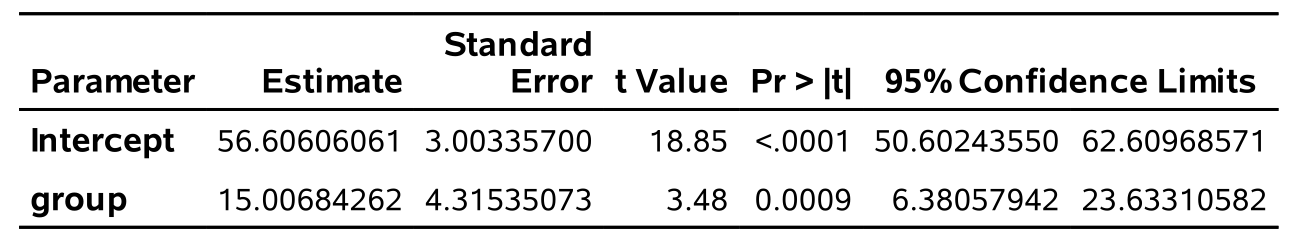
\includegraphics[width =0.9\linewidth]{img/c2/slides3-e14}
\end{center}
\bi
\item We find that $\widehat{\beta}_1=\$15$, i.e., those who pay by credit card are willing to pay $\$15$ more \textbf{on average} than those who pay with cash. 
\item This difference is statistically significant at the 5\% level ($p$-value of $0.0009$).
\item The linear regression output only reports two-sided tests, but the $p$-value for the one-sided test is half of the one reported (because of the symmetry of the Student-$t$ distribution).
\ei
\end{frame}
 
 \begin{frame}[fragile]
\frametitle{Confidence intervals}
\bi
\item 
In \SASlang, confidence intervals can be obtained by adding the option \code{clparm} to the \code{model} call. The default confidence level is $\alpha=5\%$.
\item The following code shows this for the simple linear regression model with the \code{intention} data.
\ei
\begin{align*}
\code{intention}_i = \beta_0 + \beta_1 \code{fixation}_i + \eps_i.
\end{align*}

\begin{tcolorbox}[colback=white, colframe=hecblue, title=\SASlang code to fit the regression model with the \code{glm} procedure]
\begin{verbatim}
proc glm data=infe.intention;
model intention=fixation / clparm;
run;
\end{verbatim}
\end{tcolorbox}


\end{frame}


 

\begin{frame}
\frametitle{Tests for individual parameters and confidence intervals}

\begin{center}
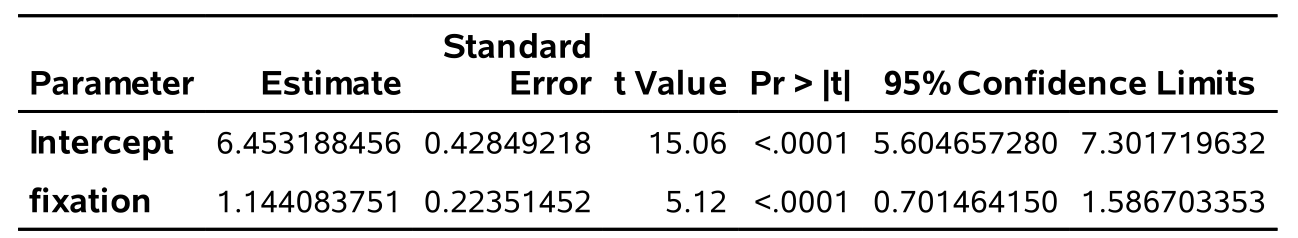
\includegraphics[width=0.9\linewidth]{img/c2/slides3-e11}
\end{center}
\bi
\item The value of the $t$-statistic for $\Hy_0: \beta_1=0$ against $\Hy_1:\beta_1 \neq 0$ is $t=1.144/0.224=5.12$.
\item The $p$-value for the two-sided test is less than $0.0001$.
\item Therefore, we reject $\Hy_0$, as there is a significant  effect of \code{fixation} on \code{intention}.
\item The $95$\% confidence interval for $\beta_1$, corresponding to the linear effect of \code{fixation}, is $[0.70; 1.59]$. 
\item Since the confidence interval does not contain the value $0$, we can conclude that the parameter is significantly different from  zero (at level $\alpha=5$\%).
\ei
\end{frame}
% 
% \begin{frame}
% \frametitle{Simple linear regression: interpretation of the test}
% \bi
% \item It turns out that when there's one explanatory variable (simple linear regression), testing the effect of the explanatory variable on the dependent variable is equivalent to testing whether the correlation between the two variables differs from 0.
% \item We've already seen that the correlation between \code{fixation} and
% \code{intention} is significant ($p$-value $p< 0.0001$). 
% \item \alert{\textbf{Careful}: this is not true when there is more than one explanatory variable in the model}.
% % \item In this case, \code{fixation} and \code{intention} appear to be linearly related. So the model is reasonable, and testing the effect of \code{fixation} on \code{intention} is justified. Some later examples will show that, just like in linear correlation, things are not always so simple.
% \ei
% \end{frame}

\begin{frame}[fragile]
\frametitle{Interpretation of the test}
 If we reject $\Hy_0: \beta_j=0$ in favor of the alternative, we rule out the possibility that there is no \textbf{linear relationship} between $\mathrm{X}_j$ and $Y$ once the effect of other variables have been factored in.
% \item Even with simple linear regression, failing to reject the null hypothesis only means there is no significant \textbf{linear} relationship between $\mathrm{X}_1$ and $Y$.

\begin{figure}
 \centering
 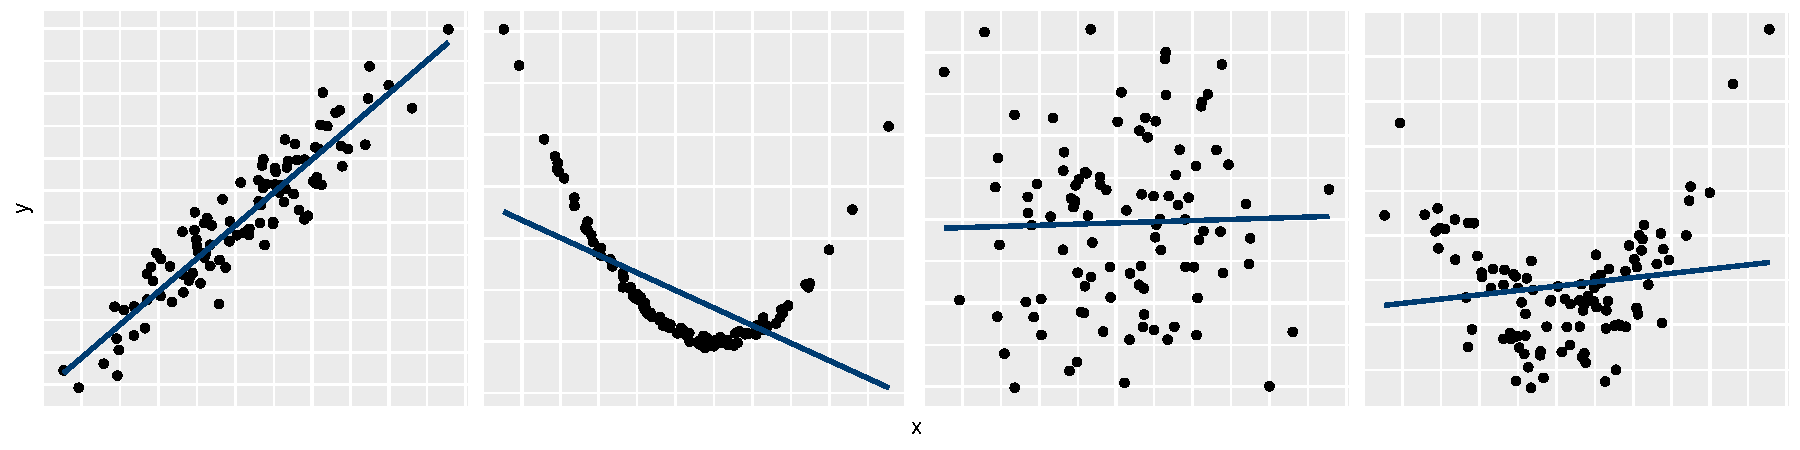
\includegraphics[width = \textwidth]{img/c2/03-linreg-fourplots}
\end{figure}
{
\footnotesize 
We reject $\Hy_0: \beta_1 = 0$ ($p$-values less than $10^{-6}$) in the two leftmost plots, but not in the two rightmost ($p$-values of 0.787 and 0.156). The coefficient of determination, from left to right, is $0.87$, $0.3$, $10^{-3}$ and $10^{-3}$.

}
\end{frame}

\begin{frame}
\frametitle{Hypothesis tests for significance of several variables}
\bi
\item There are also ways to test whether \alert{several} $\beta$'s are simultaneously equal to zero, e.g., 
\begin{align*}
\Hy_0: \beta_{\code{age}}=\beta_{\code{emotion}}=0.
\end{align*}
\item To see if we should include a categorical variable, we need to look at its \alert{global effect}.
\bi 
\item The variable \code{educ} has three levels and is modeled using two indicator variables \code{educ1} and \code{educ2}; testing the global effect of \code{educ} amounts to testing
\begin{align*}
\Hy_0: \beta_{\code{educ}_1}=\beta_{\code{educ}_2}=0.
\end{align*}
\ei
\ei
\end{frame}


\begin{frame}
\frametitle{Comparison of nested models}
\bi
\item Consider the \alert{full model} which contains $p$ predictors,
\begin{align*}
\mathbb{M}_1: Y=\beta_0+\beta_1 \mathrm{X}_1 + \cdots + \beta_g \mathrm{X}_g + \beta_{k+1}\mathrm{X}_{k+1} + \ldots + \beta_p \mathrm{X}_p + \varepsilon.
\end{align*}
\item Suppose that we want to test 
\begin{align*}
\Hy_0: \beta_{k+1}=\beta_{k+2}=\ldots=\beta_p=0.
\end{align*}
\item This hypothesis specifies that $(p-k)$ of the $\beta$ parameters are zero.
\item The \alert{restricted model} contains only the covariates for which $\beta_j \neq 0$,
\begin{align*}
\mathbb{M}_0: Y=\beta_0+\beta_1 \mathrm{X}_1 + \ldots + \beta_k \mathrm{X}_k + \varepsilon.
\end{align*}
\ei
\end{frame}



\begin{frame}[fragile]
\frametitle{Global $F$-test for testing effect of all covariates}
\bi
\item The first table output from the \SASlang \code{proc glm} procedure gives the results of the global test whether at least one of the variables in the model is useful for predicting the response variable $Y$.
\item In the model that includes all possible variables, this corresponds to testing $\Hy_0:  \beta_{\code{sex}}=\beta_{\code{age}}=\cdots =\beta_{\code{emotion}}=0$.
\begin{center}
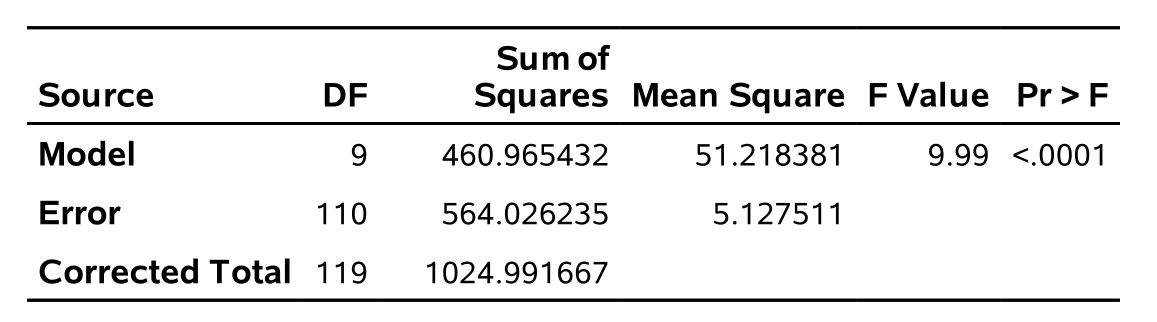
\includegraphics[width = 0.7\linewidth]{img/c2/slides3-e12}
\end{center}
\item We reject $\Hy_0$, meaning that the model contains at least one variable useful for predicting intention to buy.
\ei
\end{frame}
\begin{frame}[fragile]
\frametitle{Sum of square decomposition}
 \bi \item It is important to note that model comparisons for continuous/categorical variables are done using \textbf{Type III sum of squares}.
 \bi \item this means that the reduced model includes all but one of the explanatory variables.
 \ei \item In contrast, the Type I sum of squares table performs \textbf{sequential comparisons} with effect of covariates relative to those already included (in the order in which they entered)
 \bi \item e.g., if your first explanatory variable in the model statement is the variable of interest, the comparison is between a model with only this variable, compared to the intercept-only null model.
 \ei
 \item To avoid confusion, add \code{ss3} in the \SASlang call.
 \ei 
\end{frame}


\begin{frame}[fragile]
\frametitle{Global $F$-test for categorical variables}
\small 
\bi
% \item \SASlang also reports global tests for each of the variables.
\item When the $j$th explanatory is continuous or binary, the $F$-test is the \alert{same} as the $t$-test for $\beta_j=0$. These variables have \code{DF=1}.
\item When the variable is categorical (as defined through \code{class} in \SASlang), the output is different, e.g., the global test for a categorical variable \code{cat} with $k$ levels corresponds to the hypothesis $\Hy_0: \beta_{\code{cat}_1}=\cdots = \beta_{\code{cat}_{k-1}}=0$
\bi \item compare the model with and without the explanatory variable once other covariates are accounted for.
\ei 
\ei 
\end{frame}
\begin{frame}[fragile]
Suppose we fit a linear regression model with all the covariates for the \code{intention} data.
\begin{tcolorbox}[colback=white, colframe=hecblue, title=\SASlang code to fit the full linear model]
\begin{verbatim}
proc glm data=infe.intention noprint;
class sex educ revenue;
model intention= fixation emotion 
    sex age revenue educ / ss3 solution;
run;
\end{verbatim}
\end{tcolorbox}
\end{frame}
\begin{frame}

\bi \item 
The degrees of freedom for \code{revenue} and \code{educ} are equal to two, since each variable has three levels.
\item e.g., the $F$-test compares the model with all covariates to the one with all explanatories, but education, i.e., $\beta_{\code{educ}_1} = \beta_{\code{educ}_2}=0$.
\ei
\begin{center}
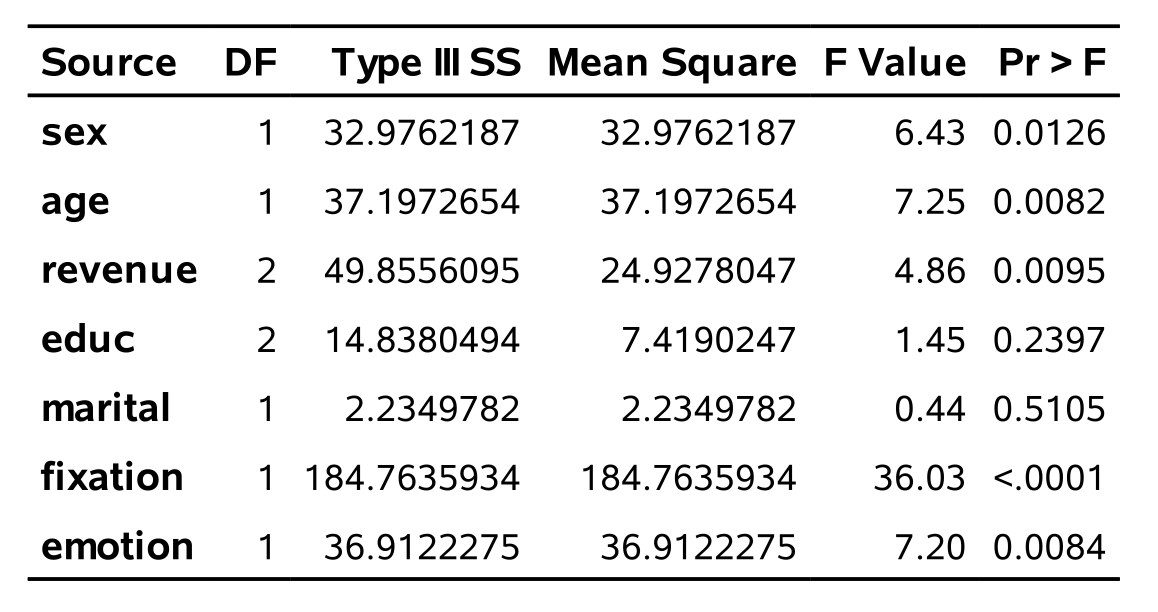
\includegraphics[width = 0.7\linewidth]{img/c2/slides3-e10.png}
\end{center}

\end{frame}

\end{document}
